\documentclass[12pt]{article}
\usepackage{amsmath, amssymb, amsthm}
\usepackage{graphicx}
\usepackage{amscd}
\usepackage{enumerate}
\usepackage{color}
\usepackage{cancel}
\usepackage{tikz}
\usepackage{empheq}
\usetikzlibrary{matrix}
\usepackage[thinlines]{easytable}
\usepackage[left=2cm,top=1.5cm,right=2cm,bottom=1cm,nohead,nofoot]{geometry}

% define an "answer box" for highlighting final answer
\definecolor{anscolor}{rgb}{.87, .77, 1}

\newlength\mytemplen
\newsavebox\mytempbox

\makeatletter
\newcommand\ansbox{%
    \@ifnextchar[%]
       {\@ansbox}%
       {\@ansbox[0pt]}}

\def\@ansbox[#1]{%
    \@ifnextchar[%]
       {\@@ansbox[#1]}%
       {\@@ansbox[#1][0pt]}}

\def\@@ansbox[#1][#2]#3{
    \sbox\mytempbox{#3}%
    \mytemplen\ht\mytempbox
    \advance\mytemplen #1\relax
    \ht\mytempbox\mytemplen
    \mytemplen\dp\mytempbox
    \advance\mytemplen #2\relax
    \dp\mytempbox\mytemplen
    \colorbox{anscolor}{\hspace{1em}\usebox{\mytempbox}\hspace{1em}}}

\makeatother

% DOCUMENT BEGINNING %
\begin{document}

\begin{center}
    Problem Set 1
\end{center}

\section*{Section 1.2}
\subsection*{Problem 23}
\[\cos(\beta) = \frac{w_1}{\vert \vert \boldsymbol{w} \vert \vert} \]

\[\sin(\beta) = \frac{w_2}{\vert \vert \boldsymbol{w} \vert \vert} \]

\[
\cos(\theta)
= \cos(\beta - \alpha)
= \cos(\beta)\cos(\alpha) + \sin(\beta)\sin(\alpha) 
\]
\[
=   \frac{v_1}{\vert \vert \boldsymbol{v} \vert \vert}
\cdot \frac{w_1}{\vert \vert \boldsymbol{w} \vert \vert}
+ \frac{v_2}{\vert \vert \boldsymbol{v} \vert \vert}
\cdot \frac{w_2}{\vert \vert \boldsymbol{w} \vert \vert}
\]
\[
=   \frac{v_1 \cdot w_1 + v_2 \cdot w_2}
{\vert \vert \boldsymbol{w} \vert \vert \; \vert \vert \boldsymbol{v} \vert \vert}
\]
\[
=   \frac{\boldsymbol{v} \cdot \boldsymbol{w}}
{\vert \vert \boldsymbol{w} \vert \vert \; \vert \vert \boldsymbol{v} \vert \vert}
\]

\subsection*{Problem 28}
The vectors lie along a line since the dot product is a linear equation. Thus, all solutions lie along a line that satisfies, $x + 2y = 5$.
~\\
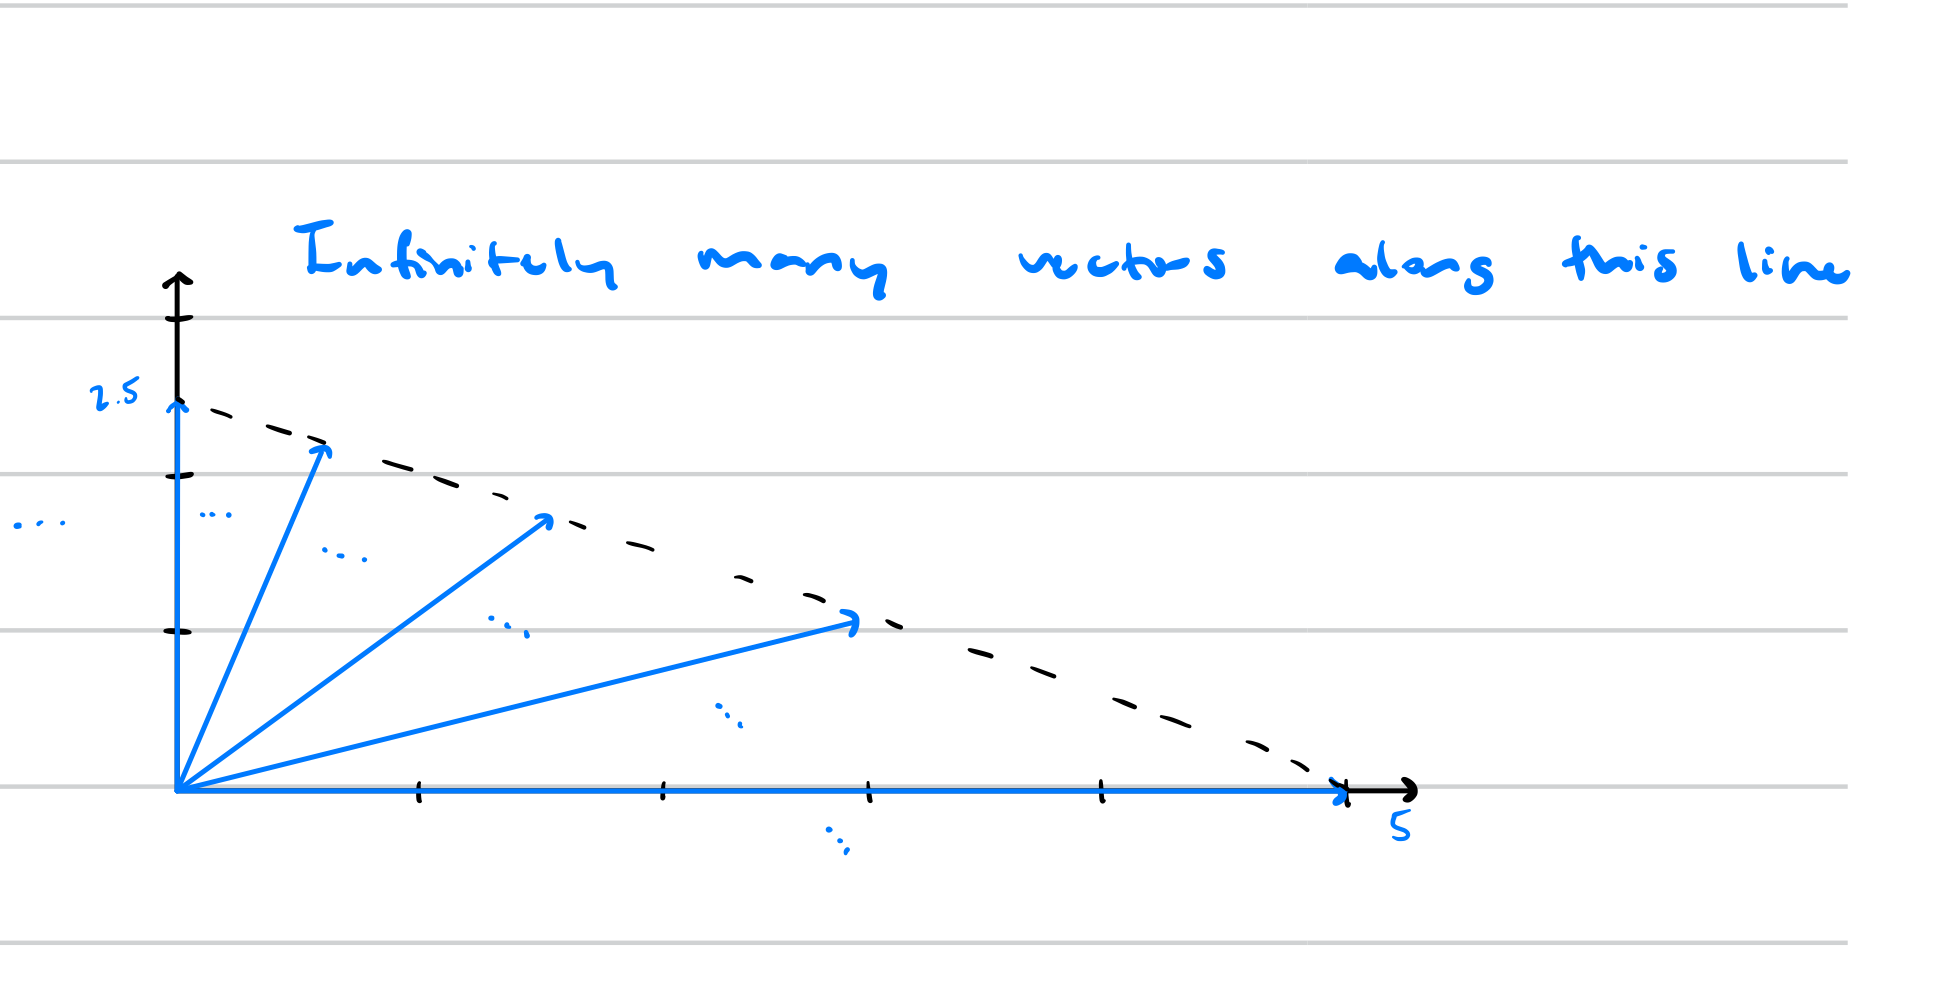
\includegraphics[scale=0.25]{s12p28a.png}

\noindent The shortest $\boldsymbol{w}$ is the vector that is perpendicular to this line. You may be able to intuit this answer to be $\boldsymbol{w} = \begin{bmatrix} 1 \\ 2 \end{bmatrix}$, but you can explicity solve for it. From the below diagram, you should be able to prove to yourself (through highschool geometry) that the smaller triangle formed by $\boldsymbol{w}$ has the same angles as the larger triangle formed by the line satisfying $x + 2y = 5$. We can use this relationship to solve for $\boldsymbol{w}$. (Remember that $\boldsymbol{w} = \begin{bmatrix} x \\ y \end{bmatrix}$)

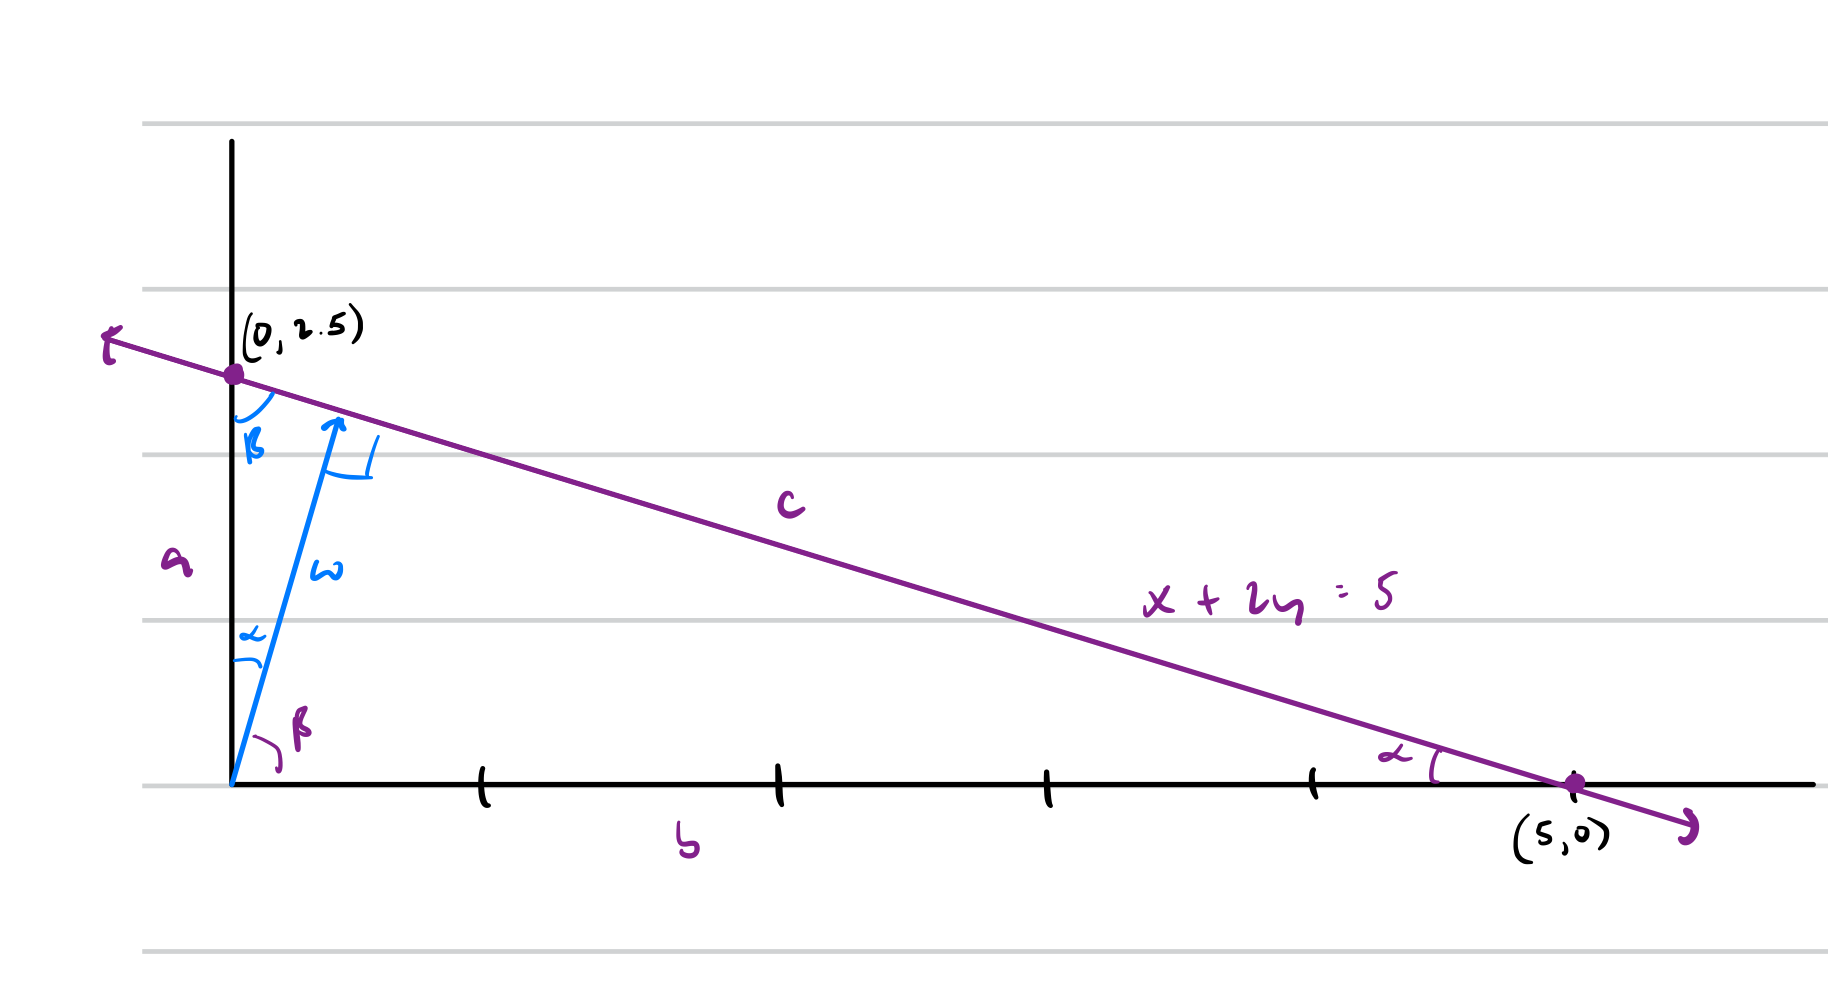
\includegraphics[scale=0.25]{s12p28b.png}

\[a = \frac{5}{2} \; \; \; \; \; \; b = 5 \; \; \; \; \; \; c = \sqrt{a^2 + b^2} 
    = \sqrt{\frac{5}{2}^2 + 5^2} 
    = \sqrt{\frac{25}{4} + 25}
    = \sqrt{\frac{125}{4}}
    = \frac{5\sqrt{5}}{2}
\]
\[
    \cos(\alpha) = \frac{b}{c} 
    = \frac{5}{\frac{5\sqrt{5}}{2}}
    = \frac{2}{\sqrt{5}}
\] 
\[ 
    \sin(\alpha) = \frac{a}{c}
    = \frac{\frac{5}{2}}{\frac{5\sqrt{5}}{2}}
    = \frac{1}{\sqrt{5}}
\]
\[
    \vert \vert \boldsymbol{w}_{min} \vert \vert 
    = \frac{5}{2} \cos(\alpha) 
    = \frac{5}{2} \cdot \frac{2}{\sqrt{5}} 
    = \frac{5}{\sqrt{5}} = \sqrt{5}
\]
\[ 
    x = \vert \vert \boldsymbol{w}_{min} \vert \vert  \sin(\alpha)
    = \frac{1}{\sqrt{5}} \sqrt{5} = 1
\]
\[
    y = \vert \vert \boldsymbol{w}_{min} \vert \vert  \cos(\alpha)
    = \frac{2}{\sqrt{5}} \sqrt{5} = 2
\]

\section*{Section 1.3}

\subsection*{Problem 4}
From the vectors we have the following 3 equations since $x_1 = 1$.
\[
    1 + 4x_2 + 7x_3 = 0 \; \; \; \; \; 
    2 + 5x_2 + 8x_3 = 0 \; \; \; \; \; 
    3 + 6x_2 + 9x_3 = 0
\]
We begin solving this sytem by adding $3 + 6x_2 + 9x_3 = 0$ and $\frac{-3}{2}(1 + 4x_2 + 7x_3 = 0)$ to find that $\frac{3}{2} - \frac{3}{2}x_3 = 0$. Thus, $x_3 = 1$. Substituting $x_3$ back into one of the original equations yields $3 + 6x_2 + 9(1) = 0$. Thus, $x_2 = -2$. Hence, the final solution is $x_1 = 1, x_2 = -2, x_3 = 1$. 
\subsection*{Problem 13}


\section*{Section 2.1}

\subsection*{Problem 29}
\[ 
\boldsymbol{u}_2
=   \begin{bmatrix} .8 & .3 \\ .2 & .7 \end{bmatrix}
    \begin{bmatrix} .8 \\ .2 \end{bmatrix}
= \begin{bmatrix} .8 \cdot .8 + .3 \cdot .2 \\ .8 \cdot .2 + .2 \cdot .7 \end{bmatrix}
= \begin{bmatrix} .64 + .06 \\ .16 + .14 \end{bmatrix}
= \begin{bmatrix} .7 \\ .3 \end{bmatrix}
\]
\[ 
\boldsymbol{u}_3
=   \begin{bmatrix} .8 & .3 \\ .2 & .7 \end{bmatrix}
    \begin{bmatrix} .7 \\ .3 \end{bmatrix}
= \begin{bmatrix} .7 \cdot .8 + .3 \cdot .3 \\ .7 \cdot .2 + .3 \cdot .7 \end{bmatrix}
= \begin{bmatrix} .56 + .09 \\ .14 + .21 \end{bmatrix}
= \begin{bmatrix} .65 \\ .35 \end{bmatrix}
\]

\subsection*{Problem 30}
You can see that both vectors converge to $\begin{bmatrix} 0.6 \\ 0.4 \end{bmatrix}$.

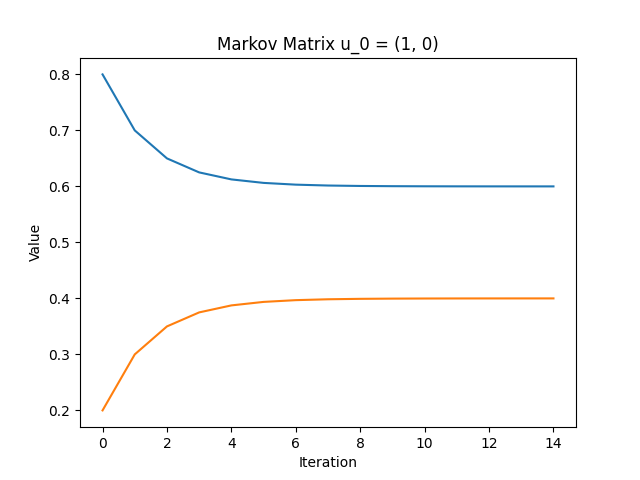
\includegraphics[scale=0.55]{s21p30a.png}
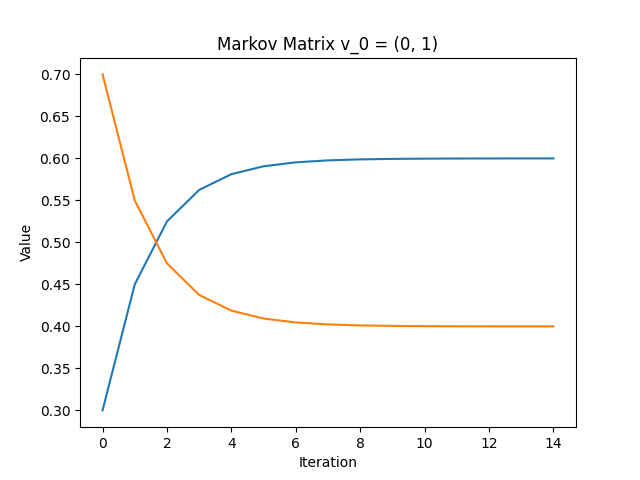
\includegraphics[scale=0.55]{s21p30b.png}

\noindent We can prove this by showing that $\begin{bmatrix} 0.6 \\ 0.4 \end{bmatrix}$ does not change when multiplied by our Markov Matrix.

\begin{center}
    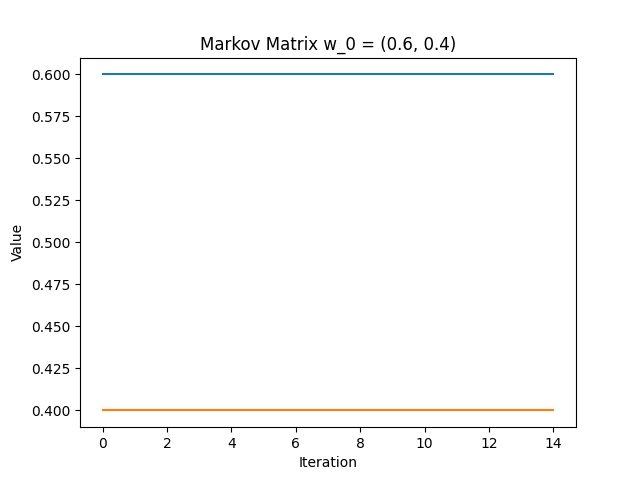
\includegraphics[scale=0.75]{s21p30c.png}
\end{center}

\section*{Section 2.2}

\emph{Three planes can fail to have an intersection point, even if no planes are parallel. The system is singular if row 3 of $A$ is a \textbf{linear combination} of the first two rows.}

\section*{Section 2.3}

\section*{Section 2.4}

\section*{Section 2.5}

\end{document}